
%%%%%%%%%%%%%%%%%%%%%%%%%%%%%%%%%%%%%%%%%%%%%%%%%%

%%%%%%%%%%%%%%%%% APPENDICES %%%%%%%%%%%%%%%%%%%%%

\appendix

\section{Tidal torque \& Equations of motion}
\label{app:eom}

In this appendix, we derive the equations of motion used to simulate the asteroid angular velocity during the encounter. In particular, we describe our coordinates (section \ref{sec:coordinates}) for an encountering asteroid's position and orientation, and we parametrize its density distribution via its ``density moments'' (section \ref{sec:moments}). Then we derive an arbitrary-order equation for tidal torque (section \ref{sec:tidal-torque}) and write the equations of motion for the system (section \ref{sec:eom}). We do not consider any third-body perturbations, and we assume that the body being encountered (the central body, e.g.~a planet) is much more massive than the asteroid.

\subsection{Coordinates}
\label{sec:coordinates}

We make use of two frames of reference to model this system. One is the ``inertial frame,'' with axes denoted by $\unit{X}$, $\unit{Y}$, $\unit{Z}$ and origin placed at the central body's centre of mass. $\unit{X}$ points from the central body to the asteroid periapse, and $\unit{Z}$ points parallel to the orbit angular momentum. We assume that the mass distribution of the central body is known in this inertial frame.

Our second frame is the ``body-fixed'' frame, denoted by $\unit{x}, \unit{y}, \unit{z}$. Each axis in this frame is aligned with a principal axis and rotates with the asteroid, with its origin at the asteroid's centre of mass. For definiteness, we define $\unit{z}$ to be the principal axis with maximal moment of inertia (this is the short axis mode, to use the vocabulary of Ref.~\cite{kaasalainen2001interpretation}). In general, we use capital letters to denote vectors in the inertial frame and lowercase vectors to denote vectors in the body-fixed frame.

The difference between the origins of the body-fixed and inertial frames is the position of the asteroid. We represent the relative orientations by $z-y-z$ Euler angles $\alpha$, $\beta$, and $\gamma$, such that a matrix $M$ rotating from the body-fixed to the inertial frame ($M\bm{r} = \bm{R}$) is given by
\begin{equation}
M = R_z(\alpha) R_y(\beta) R_z(\gamma).
\label{eqn:euler-angles}
\end{equation}
Here, $R_i(\theta)$ is a rotation around the unit vector $i$ by $\theta$ (figure \ref{fig:euler-angles}).

\begin{figure}
    \centering
    \begin{tikzpicture}
    \draw[-{Latex[length=3mm]}] (0, 0) -- (-4, 0) node[anchor=east] {$\unit x$};
    \draw[-{Latex[length=3mm]}] (0, 0) -- (2, -3) node[anchor=west] {$\unit y$};
    \draw[-{Latex[length=3mm]}] (0, 0) -- (0, 4) node[anchor=south] {$\unit z$};
    \draw[dashed, -{Latex[length=3mm]}] (0, 0) -- (3.7, -2) node[anchor=north] {};
    \draw[line width=0.5mm,-{Latex[length=3mm]}] (0, 0) -- (-0.5, -3) node[anchor=north] {$\unit X$};
    \draw[line width=0.5mm,-{Latex[length=3mm]}] (0, 0) -- (4, 1) node[anchor=south] {$\unit Y$};
    \draw[line width=0.5mm,-{Latex[length=3mm]}] (0, 0) -- (-1.6, 2.7) node[anchor=south] {$\unit Z$};
    \draw[->] (0.5, -0.75) arc (290:302:2.5);
    \draw (0.9, -0.9) node[anchor=center] {$\alpha$};
    \draw[->] (0, 1.2) arc (130:161:1.3);
    \draw (-0.3, 1.3) node[anchor=center] {$\beta$};
    \draw[->] (0.97, -0.52) arc (330:368:1.3);
    \draw (1.4, -0.25) node[anchor=center] {$\gamma$};
    %\draw[-{Latex[length=3mm]}] (0, 0) -- (0, 4) node[anchor=south] {$\unit Z$};
    %\draw[-{Latex[length=3mm]}] (0, 0) -- (4, 0) node[anchor=west] {$\unit Y$};
    %\draw[-{Latex[length=3mm]}] (0, 0) -- (-2, -2) node[anchor=east] {$\unit X$};
    \end{tikzpicture}
    \caption{$z-y-z$ Euler angles used in this work to express the orientation of the asteroid. Orientation is expressed as a rotation from the body-fixed axes (lowercase) to the inertial axes (bold and uppercase). The origins are co-located for demonstration purposes.}
    \label{fig:euler-angles}
\end{figure}


\subsection{Density moments}
\label{sec:moments}

In the next section, it will be shown that only certain parameters of the asteroid density distribution affect tidal torque called ``density moments.'' First, we define the un-normalized spherical harmonics $Y_{\ell m}(\theta, \phi) = P_{\ell m}(\cos \theta)e^{im\phi}$, where $P_{\ell m}$ are the associated Legendre Polynomials without the Condon-Shortley phase. The regular and irregular spherical harmonics then defined as
\begin{equation}
  \begin{split}
    S_{\ell m}(\bm r) &= (-1)^m (\ell - m)! \frac{Y_{\ell m}(\unit r)}{r^{\ell+1}} \\
    R_{\ell m} (\bm r) &= (-1)^m \frac{r^\ell}{(\ell + m)!} Y_{\ell m}(\unit r).
  \end{split}
\end{equation}
These spherical harmonics obey many useful identities summarized in Ref.~\cite{Gelderen1998TheSO}, which are also useful for quantum mechanics. They were used to define the density moments in equation \ref{eqn:klm}, which can be extended to the central body:
\begin{equation}
  \begin{split}
    &J_{\ell m} = \frac{a_\mathcal{B}^{2-\ell}}{I_\mathcal{B}} \int_\mathcal{B} d^3 r \rho_\mathcal{B}(\bm r) R_{\ell m}(\bm r)\\
  \end{split}
  \label{eqn:jlm}
\end{equation}
By contrast, $J_{\ell m}$ should be computed in the inertial frame. The length scale $a_\mathcal{B}$ and MOI scale $I_\mathcal{B}$ can be defined similarly to $a_\mathcal{A}$ and $a_\mathcal{B}$ in equations \ref{eqn:aa} and \ref{eqn:ia}, but they could also be set to any other scales of the proper units, e.g. $a_\mathcal{B}$ equal to the central body radius and $I_\mathcal{B} = \mu_\mathcal{B}a_\mathcal{B}^2$, where $\mu_\mathcal{B}$ is the central body mass.

Note that both $J_{\ell m}$ and $K_{\ell m}$ are unitless. We call them ``moments'' because the $R_{\ell m}(\bm r)$ contains an $r^\ell$ dependence so that $K_{\ell m}$ is the $\ell$th density moment of the asteroid. The gravitational potential field of the asteroid can be written entirely in terms of $K_{\ell m}$ and $a_\mathcal{A}$, so we expect not to need any information about the density distribution of the asteroid beyond these parameters to compute tidal torque.

These moments share several key properties which we discuss before continuing. Firstly, for real mass density, properties of the spherical harmonics imply that $K_{\ell m} = (-1)^m K_{\ell, -m}^*$. Therefore, the set of $K_{\ell m}$ for $\ell < \ell_\text{max}$ contains $\ell_\text{max}^2$ degrees of freedom. However, some of these degrees of freedom are redundant with the choice of coordinates: $K_{1m} = 0$ since the body-fixed frame is centred on the asteroid centre of mass. Further calculation reveals that the alignment of the body-fixed frame with the asteroid principal axes also forces $K_{21}= 0$ and $\Im K_{22}=0$. The only physical density moments for $\ell \leq 2$ are therefore $K_{22}$, $K_{20}$, and $K_{00}$. The first two are related to the moment of inertia around each principal axis by equation \ref{eqn:moi}, while $K_{00} = \mu_\mathcal{A} a_\mathcal{A}^2 / I_\mathcal{A}$ will not be relevant to this study as it does not appear in \ref{eqn:tidal-torque}. 

The physical meaning of $K_{22}$ and $K_{20}$ can also be interpreted via a special case: if the asteroid is a uniform-density triaxial ellipsoid, the moments of inertia are simple to compute in terms of the semi-axis lengths and can be compared to those found in equation \ref{eqn:moi}. This yields semi-axis lengths of 
\begin{equation}
  \begin{split}
  a &= \sqrt{\frac{5}{3}}a_\mathcal{A}\sqrt{1-2K_{20}+12K_{22}}\\
  b &= \sqrt{\frac{5}{3}}a_\mathcal{A}\sqrt{1-2K_{20}-12K_{22}}\\
  c &= \sqrt{\frac{5}{3}}a_\mathcal{A}\sqrt{1+4K_{20}}.
  \label{eqn:ellipsoid-axes}
  \end{split}
\end{equation}
The higher-order moments $K_{3m}$ can be thought of loosely as measuring the large-scale asymmetries of the asteroid. An asteroid that is mirror-symmetric along the $\unit{x}$ axis (meaning $\rho_\mathcal{A}(x,y,z)=\rho_\mathcal{A}(-x,y,z)$) necessarily sets certain density moments to zero. Which density moments are zeroed by which mirror symmetries is outlined in table \ref{tab:klm-symmetries}. All $K_{3m}$ are zeroed by at least one mirror symmetry. 

\begin{table}
  \centering
  \begin{tabular}{c|ccccccc}
    \hline
    $\ell$ & $\Re K_{\ell 3}$ & $\Im K_{\ell 3}$ & $\Re K_{\ell 2}$ & $\Im K_{\ell 2}$ & $\Re K_{\ell 1}$ & $\Im K_{\ell 1}$ & $K_{\ell 0}$ \\ \hline
    0 &  &  &  &  &  &  & -\\ 
    1 &  &  &  &  & x & y & z\\ 
    2 &  &  & - & x,y & y,z & x,z & -\\ 
    3 & x,z & y,z & z & x,y,z & x & y & z\\ \hline
  \end{tabular}
  \caption{Axes of mirror symmetry that imply zeroed density moments. For example, for mirror symmetries along $\unit y$ or $\unit z$, $\Im K_{32}=0$. Mirror symmetry along $\unit x$ means $\rho_\mathcal{A}(x, y, z) = \rho_\mathcal{A}(-x, y, z)$. Dashes indicate that none of the mirror symmetries zero the moment in question. Since $r^2>0$ for $r\neq 0$, no symmetries set $a_\mathcal{A}=0$ either.}
  \label{tab:klm-symmetries}
\end{table} 

Finally, the requirement that $\rho_\mathcal{A}(\bm r) \geq 0$ everywhere restricts $K_{\ell m}$. In the case of $K_{2m}$, this fact and the constraint that $I_z$ is larger than $I_x$ or $I_y$ requires $K_{20}$ and $K_{22}$ to fall in the triangle
\begin{equation}
  -\frac{1}{4} \leq K_{20} \leq 0, \qquad |K_{22}| \leq -\frac{K_{20}}{2}.
  \label{eqn:parameter-bounds}
\end{equation}
An analytical constraint on $K_{3m}$ based on this property is more difficult to derive, but in practice, we also observe that $|K_{3m}| < 0.01$.




\subsection{Tidal torque}
\label{sec:tidal-torque}

Derivations for the tidal torque experienced by a rigid body in the gravitational field of a larger mass have been computed by several previous studies \cite{paul88,HouMar2017,BOUE2009750, ashenberg07}, often in terms of the moment of inertia of the rigid body (or higher order moments of inertia), and to varying degrees of precision. A simple, first-order derivation is also easily computable in terms of the asteroid moment of inertia in the inertial frame.

Here, we present a new derivation of the tidal torque to arbitrary orders in terms of the density moments of an asteroid defined in section \ref{sec:moments}. These density moments can be pre-computed and do not have to be re-evaluated every time-step.

Throughout this paper, we assume that the asteroid remains rigid throughout the encounter. We also assume no third-body perturbations from other Solar System objects. (More accurately, we assume that all third-body perturbing objects lie closer to the central body's centre of mass than the asteroid perigee distance so that their density moments can be included in the density moments of the central body.) For the sake of simplicity, we also assume that the density moments of the central body are known and do not evolve with time (i.e., the central body's rotation is marginal compared to the timescale of the encounter).

The gravitational potential energy of the central body is, in its most general form,
\begin{equation}
V(\bm R') = -G\int_\mathcal{B} d^3 R \rho_\mathcal{B}(\bm R) \frac{1}{|\bm{R}-\bm{R'}|}.
\label{eqn:first-pe}
\end{equation}
where $\rho_\mathcal{B}$ is the density distribution of the central body and $\mathcal{B}$ indicates the central body's volume. All vectors here are written in the inertial frame. Given $|\bm{R}| < |\bm{R'}|$, Ref.~\cite{Gelderen1998TheSO} gives the identity
\begin{equation}
  \frac{1}{|\bm R - \bm R'|} = \sum_{\ell, m} R_{\ell m}(\bm R) S_{\ell m}^*(\bm R'),
  \label{eqn:ylm-expansion}
\end{equation}
where the sum is shorthand for $\sum_{\ell, m} = \sum_{\ell = 0}^\infty \sum_{m=-\ell}^\ell$.
We are interested in translating the potential energy of equation \ref{eqn:first-pe} to the body-fixed frame. To do this, we let $\bm{R'} = \bm D + \bm U$, where $\bm D$ is the location of the asteroid in the inertial frame. We further define $\bm U = M\bm u$, where $\bm u$ is in the body-fixed frame and $M$ is the rotation matrix given by the Euler angles $\alpha$, $\beta$, and $\gamma$ (see section \ref{sec:coordinates}). The translation from $\bm {R'}$ to $\bm U$ is then attained by the identity 
\begin{equation}
  S_{\ell m}(\bm R') = \sum_{\ell', m'} (-1)^{\ell'}R^*_{\ell' m'}(\bm U)S_{\ell+\ell', m + m'} (\bm D),
  \label{eqn:ylm-translation}
\end{equation}  
provided by Ref.~\cite{Gelderen1998TheSO}, and from $\bm U$ to $\bm u$ is given by
\begin{equation}
  \begin{split}
    Y_{\ell m}(M\bm u) = \sum_{m'=-\ell}^\ell & (-1)^{m+m'}\sqrt{\frac{(\ell-m')!(\ell+m)!}{(\ell+m')!(\ell-m)!}} \\
    & \times \mathcal{D}^\ell_{mm'}(M)^* Y_{\ell m'}(\bm u).\\
  \end{split}
  \label{eqn:ylm-rotation}
\end{equation}
Here, $\mathcal{D}^\ell_{mm'}(M)$ are the Wigner-$D$ matrices, which are determined by the Euler angles $\alpha$, $\beta$, and $\gamma$ of $M$.

Equations \ref{eqn:first-pe} to \ref{eqn:ylm-rotation} then provide formula for $V(\bm u)$ expressed as a sum of integrals over $\mathcal{B}$ of the central body density $\rho_\mathcal{B}(\bm R)$ times $R_{\ell m}(\bm R)$. These are expressed via equation \ref{eqn:jlm} as $J_{\ell m}$.

The tidal torque experienced by the asteroid (in the body-fixed frame) is given by
\begin{equation}
  \bm{\tau}(\bm u) = \int_\mathcal{A} d^3 u \rho_\mathcal{A}(\bm u) (\bm u \times (-\nabla_{\bm u} V(\bm u)))
\end{equation}
where $\rho_\mathcal{A}$ is the density distribution of the asteroid and $\mathcal{A}$ indicates the volume of the asteroid. Making use of one more identity concerning the derivatives of spherical harmonics:
\begin{equation}
  \begin{split}
  \bm u \times \nabla R_{\ell m}(\bm u)=&\frac{1}{2}\Big[(i\unit x - \unit y)(\ell-m+1)R_{\ell,m-1}(\bm u)\\
  &+(i\unit x+\unit y)(\ell+m+1)R_{\ell,m+1}(\bm u)\\
  & +2im\unit z R_{\ell m}(\bm u)\Big],
  \end{split}
\end{equation}
tidal torque can now be expressed as a function only of the constants $J_{\ell m}$, $K_{\ell m}$, $a_\mathcal{A/B}$, $I_\mathcal{A/B}$, and the asteroid orientation and position (equation \ref{eqn:tidal-torque}). Some $K_{\ell m}$ terms are written in this equation with $|m|>\ell$; these should all be taken to be zero.

Equation \ref{eqn:tidal-torque} possesses a few explicit properties. Firstly, $\bm \tau$ is independent of asteroid mass. The mean density of the asteroid is therefore not constrained by tidal torque analysis. Secondly, torque is largest when $D$ is small (as expected), with the leading order of $\bm \tau$ proportional to $D^{-3}$. Thirdly, each $J_{\ell m}K_{\ell' m'}$ term is multiplied by $(a_\mathcal{B}/D)^\ell (a_\mathcal{A}/D)^{\ell'}$, the latter of which especially is small in most cases. Equation \ref{eqn:tidal-torque} can therefore be computed approximately by removing terms of large $\ell$ and $\ell'$. For our analysis, we removed $\ell' > 3$ and we usually keep only $\ell=0$. Note that $\ell=1$ contributes nothing since $J_{1m}=0$. $J_{2m}$ measures the oblaneness and its effects are studied in appendix \ref{app:uncertainty-dependence}.

Further insight can be gained by remarking the value of the first-order of $\bm \tau$ for particular Euler angle cases. Setting $\beta = 0$ produces diagonal Wigner-$D$ matrices, and hence $\bm \tau \parallel \unit z$ to first-order. Also, the component $\tau_z$ oscillates, so that for certain values of $\alpha$ and $\gamma$, $\bm \tau = 0.$ This $\beta=0$ condition is equivalent to $\unit z \parallel \unit Z$ (see figure \ref{fig:euler-angles}).

For $\beta = \pi/2$, there are two interesting cases. One is for $\alpha = \phi$ (or $\alpha = \pi + \phi$), where $\phi$ is the angle between the asteroid and the perigee. In this case, $\tau = 0$ to first-order. The second case is $\alpha = \phi \pm \pi/2$, when again $\bm \tau \parallel \unit z$ and $\tau_z$ oscillates. At perigee ($\phi=0$), these conditions are equivalent to $\unit z \parallel \unit X$ and $\unit z \parallel \unit Y$ respectively.

The $\bm \tau \parallel \unit z$ cases are interesting because they do not induce tumbling. If velocity is $\bm \omega \parallel \unit z$ (a non-tumbling state, since $\unit z$ is a principal axis), then $\bm \omega \parallel \bm L$ and $\bm \tau = \dot{\bm L} \parallel \dot{\bm \omega}$ so that $\bm \omega$ remains parallel to $\unit z$ and non-tumbling. These cases of torque are additionally significant because not as many terms contribute to $\tau_z$ as to $\tau_x$ and $\tau_y$.

\subsection{Equations of motion}
\label{sec:eom}


The equations of motion of the asteroid position $\bm D$ are given by Newton's law of gravitation
\begin{equation}
  \dot{\bm V} = -\frac{G \mu_\mathcal{B}}{D^3} \bm D \qquad \dot{\bm D} = \bm V
  \label{eqn:pos-eom}
\end{equation}
where $\bm V$ is the asteroid velocity in the inertial frame. Rather than derive equations of motion for the Euler angles (which suffer from gimbal lock), we instead represent the orientation of the asteroid with a quaternion $\quat q$ which can be converted into Euler angles to compute $\mathcal{D}(\alpha, \beta, \gamma)$. This quaternion evolves as 
\begin{equation}
  \dot{\quat q} = \frac{1}{2}\quat q\quat \omega.
  \label{eqn:quat-eom}
\end{equation}
for angular velocity $\bm \omega$ given in the body-fixed frame. The equations of motion of $\bm \omega$ in turn are given by
\begin{equation}
  \begin{split}
    I_x \dot \omega_1 - \omega_y \omega_z (I_y - I_z) &= \tau_x\\
    I_y \dot \omega_2 - \omega_z \omega_x (I_z - I_x) &= \tau_y\\
    I_z \dot \omega_3 - \omega_x \omega_y (I_x - I_y) &= \tau_z.
  \end{split}
  \label{eqn:omega-eom}
\end{equation}
Equations \ref{eqn:tidal-torque}, \ref{eqn:moi}, and \ref{eqn:pos-eom} to \ref{eqn:omega-eom} form a set of non-linear, first-order coupled differential equations in which can be numerically integrated. They are expressed in terms of the constant physical parameters $I_\mathcal{A/B}$, $a_\mathcal{A/B}$, $J_{\ell m}$, and $K_{\ell m}$.

Note that equation \ref{eqn:omega-eom} is independent of $a_\mathcal{A}$ to first-order in $\bm \tau$, because $I_{j} \propto a_\mathcal{A}^2$ for all $j$ and $\bm \tau \propto a_\mathcal{A}^2$. Therefore, scaling $a_\mathcal{A}$ merely scales the value of the sub-leading-order contributions to $\bm \tau$.




\section{Reference asteroid configurations}
\label{app:reference-configs}

Except when otherwise mentioned, we use the following asteroid encounter parameters. Many of the parameter choices are made to maximize the quality of observations (a close orbit, large asteroid, etc.) This is so that our analysis is most sensitive to the affect changing these parameters to the methodology's output.

\begin{enumerate}
  \item An orbit around a spherical, Moonless Earth with $6$ km s$^{-1}$ excess velocity and perigee at 5 Earth radii. This orbit was chosen to roughly match that of 99942 Apophis \cite{giorgini2005recent, giorgini2008predicting, smalley20052004}, discovered on June 19, 2004 by R. A. Tucker, D. J. Tholen, and F. Bernardi. These orbital parameters correspond to an eccentricity of 3.88. The comparison to Apophis is complicated by the fact that Apophis is smaller than our $a_\mathcal{A}$ value, is tumbling \cite{PRAVEC201448}, and may change slightly in physical properties due to tidal interaction during the encounter \cite{yu2014numerical,hirabayashi2021finite}. Further work must therefore be done to apply this analysis to Apophis. 
  \item An initial roll of $\gamma_0=\pi/8$.
  \item A cadence of 2 minutes and observational uncertainty of $\sigma_\theta = 0.01$ and $\sigma_P / P = 10^{-7}$.
  \item A rotational period of 9 hours, with the angular velocity vector distributed between the $\unit X$, $\unit Y$, and $\unit Z$ axes in a $1:2:-2$ ratio.
  \item An asteroid with radius $a_\mathcal{A} = 1$ km and $K_{3m}=0$. For $K_{22}$ and $K_{20}$, we use two standard values: one with $(K_{22}, K_{20}) = (0, -0.097)$ and one with $(0.052, -0.202)$. Including the third point obtained by reflection $K_{22}\rightarrow -K_{22}$, these are the three points that minimize the mean distance between an arbitrary point in the allowed parameter space (equation \ref{eqn:parameter-bounds}) and these reference values. The first point is called the symmetric case because the corresponding uniform-density-ellipsoid model is rotationally symmetric around $\unit z$. The second case and its reflection are called the asymmetric cases. Values of $(0.052, -0.202)$ have $a < b$ in the ellipsoid model, and the reflected value has $a > b$. If not specified, we use the $a < b$ case. Specifically, the asymmetric case has $a=1140$ m, $b=1839$ m, and $c=565$ m, while the symmetric case has $a=b=1411$ m and $c=1008$ m.
\end{enumerate}

The surface of a spherical asteroid with this rotational period and $a_\mathcal{A}$ rotates at $\SI{25}{\centi\meter\per\second}$ at the equator. The asymmetric and symmetric ellipsoids have maximum equatorial velocities of $\SI{36}{\centi\meter\per\second}$ and $\SI{27}{\centi\meter\per\second}$ respectively.


\section{Additional density distribution models}
\label{app:more-models}

Two models were discussed in section \ref{sec:density-distro} to translate density moment constraints into density distribution constraints. Here we outline two additional models, the nearly-uniform and the harmonic models, which are less conventional but still useable for extracting density distribution properties. Unlike the finite element and lumpy models discussed in the main text, these models will yield smooth distributions with no discrete transitions. They also rely on a known surface for the asteroid.

\subsection{Nearly-uniform model}
In this nearly-uniform model, we seek to pick one density distribution from the many distributions consistent with the data by maximizing a prior distribution $f[\rho(\bm r)]$, which can be chosen manually. Any prior distribution can be chosen, but the following prior is both interesting and numerically efficient.

As part of our prior, we require that the asteroid density distribution satisfy $I_\mathcal{A} = \mu_\mathcal{A} a_\mathcal{A}^2$. This constraint is desirable as it encourages nearly uniform density distributions; recall that a perfectly uniform asteroid always satisfies this constraint. To define the prior, we divide the asteroid into $n \gg 1$ small regions of volume $V$, each with position $\bm r_i$ and density $\rho_i = \delta_i + 1$. Setting the mass of the asteroid equal to its volume, the average density is 1, so $\delta_i$ is the difference between the average and local density. We set $f[\rho(\bm r)]$ to be a multivariate-Gaussian distribution on $\delta_i$ centred on zero to minimize non-uniformity, i.e.
\begin{equation}
  f[\rho(\bm r)] \propto \prod_i \exp\parens{-\frac{\delta_i^2}{2\sigma^2}} \implies \ln f[\rho(\bm r)] \simeq -\sum_i \delta_i^2
  \label{eqn:nu-f}
\end{equation}
where $\sigma$ is an irrelevant constant. The density moments, MOI scale, and mass are 
\begin{equation}
  K_{\ell m} = \frac{V}{\mu_\mathcal{A}a_\mathcal{A}^{\ell}} \sum_i (\delta_i + 1) R_{\ell m}(\bm r_i)
  \label{eqn:nu-klm}
\end{equation}
\begin{equation}
  I_\mathcal{A} = \mu_\mathcal{A} a_\mathcal{A}^2 = V \sum_i (\delta_i + 1) r_i^2
  \label{eqn:nu-ia}
\end{equation}
\begin{equation}
  \mu_\mathcal{A} = V\sum_i (\delta_i + 1) \implies 0 = \sum_i \delta_i.
  \label{eqn:nu-mass}
\end{equation}
Writing $\delta_i$ as an $n$-dimensional vector $\bm \delta$, equation \ref{eqn:nu-klm} is a matrix equation for $K_{\ell m}$ and equations \ref{eqn:nu-ia} and \ref{eqn:nu-mass} are vector dot product equations. Combining $K_{\ell m}$, $I_\mathcal{A}$, and $0$ into a single vector $\bm K$, these equations can be written as a single underdetermined matrix equation we denote as $\bm K = M \bm \delta + \bm C$, where the components of constant matrix $M$ and constant vector $\bm C$ are known given a fixed layout of the $n$ regions. Some of the components of $\bm K$, such as $I_\mathcal{A}$, $\mu_\mathcal{A}$, and $K_{1m}$, are constraints. We treat the other components as parameters of the model. The task is then to find $\bm \delta$ that satisfies this matrix equation and maximizes $f(\bm \delta)$. But the form of equation \ref{eqn:nu-f} shows that the maximum of $\ln f$ (and the maximum of $f$) is the minimum of $|\bm \delta|^2$. The value of $\bm \delta$ that obeys the constraints and minimizes its norm is given by the Moore-Penrose inverse:
\begin{equation}
  \bm \delta = M^+ (\bm K - \bm C); \qquad M^+ = M^\dagger(M M^\dagger)^{-1}
  \label{eqn:nu-delta}
\end{equation}
where $M^\dagger$ is the adjoint of $M$.

The probability distribution of $\bm K$ is given by the output of the fit described in section \ref{sec:fit}. The parameters of this model, $\bm K$, might differ from this distribution due to the additional constraint that the density fall in realistic values. This can be implemented by individually checking the components $\bm \delta$ computed by equation \ref{eqn:nu-delta} and confirming that $1 + \delta_i$ lies within the acceptable range of densities.


\subsection{Harmonic model}
For the harmonic model, we limit ourselves to density distributions that are harmonic; i.e., they satisfy $\nabla^2 \rho(\bm r) = 0$. We have no physical justification for why this assumption should be true, but it is useful as a simplification to gain qualitative insight into the properties of the asteroid density distribution.

A harmonic density distribution can be expanded in terms of the spherical harmonics as $\rho(\bm r) = \sum_{\ell m} C_{\ell m} R_{\ell m}(\bm r)^*$ where $C_{\ell m}$ are complex, free parameters. This series can be truncated at some maximum $\ell$. The density moments, MOI scale, and mass can then be explicitly computed as a function of $C_{\ell m}$:
\begin{equation}
  K_{\ell m} = \frac{a_\mathcal{A}^{2-\ell}}{I_\mathcal{A}} \sum_{\ell m} C_{\ell' m'} \int_\mathcal{A} d^3 r R_{\ell' m'}(\bm r)^* R_{\ell m}(\bm r)
  \label{eqn:harmonic-klm}
\end{equation}
\begin{equation}
  I_\mathcal{A} = \sum_{\ell m} C_{\ell m} \int_\mathcal{A} d^3 r R_{\ell m}(\bm r)^* r^2
  \label{eqn:harmonic-ia}
\end{equation}
\begin{equation}
  \mu_\mathcal{A} = \sum_{\ell m} C_{\ell m} \int_\mathcal{A} d^3 r R_{\ell m}(\bm r)^*.
  \label{eqn:harmonic-mass}
\end{equation}
These integrals can be pre-computed given a known asteroid shape $\mathcal{A}$, so that computing $C_{\ell m}$ to match a given $K_{\ell m}$ is fast. Furthermore, their values when $\mathcal{A}$ is spherical gives us insight into the influence of $K_{\ell m}$ on density distributions. In this case, $I_\mathcal{A} \propto C_{00}$ and the integral of equation \ref{eqn:harmonic-klm} is nonzero only when $\ell' = \ell$ and $m'=m$. Therefore, $C_{\ell m}$ is proportional to $K_{\ell m}$. The density distribution can be immediately visualized given the density moments as a sum of the solid spherical harmonics weighted by $K_{\ell m}$. When the asteroid is non-spherical, the shape itself contributes to $K_{\ell m}$ so as to break this picture.

Imposing constraints on these moments is also necessary. The choice of mass is enforced merely by enforcing equation \ref{eqn:harmonic-mass}. We impose bounds on $\rho(\bm r)$ by acknowledging that harmonic functions such as $\rho(\bm r)$ in a region such as $\mathcal{A}$ attain their maxima on the boundary of the region, so that it is only necessary to ensure that $\rho$ lies within the allowed range on the asteroid boundary rather than within the entire asteroid. This can be done by parametrizing the asteroid surface as a function of two variables and minimizing and maximizing $\rho$ with respect to those variables, ensuring these minima and maxima are within the allowed range.



\section{The cadence cut-off}
\label{app:cadence-tests}

\jtd{Remove this section or included it in the following section.}

In section \ref{sec:scan-cadence}, we noted that posterior uncertainty as a function of observation cadence $\Delta t$ appears to increase suddenly near $\Delta t \sim T_\text{cad}=30-40$ min. In this appendix, we discuss the location of this cadence cut-off as a function of the physical parameters of the asteroid.

In figure \ref{fig:cad-contour}, we display contour plots of posterior uncertainty $\sigma(K_{\ell m})$ of the fit parameters as a function of both cadence $\Delta t$ and $P_\omega$ (left panel) or the relative orbit speed $t_\text{spin} / t_\text{orbit}$ (right panel). Both panels show the same sudden increase in posterior uncertainty we named $T_\text{cad}$, located around the region where $\sigma_\rho / \rho = 100\%$ and now visible as a function of frequency and relative orbit speed. In all cases, the value of $\gamma_0$ was set so that all data points achieve the same value of $\gamma$ at perigee.

\begin{figure*}
  \centering
  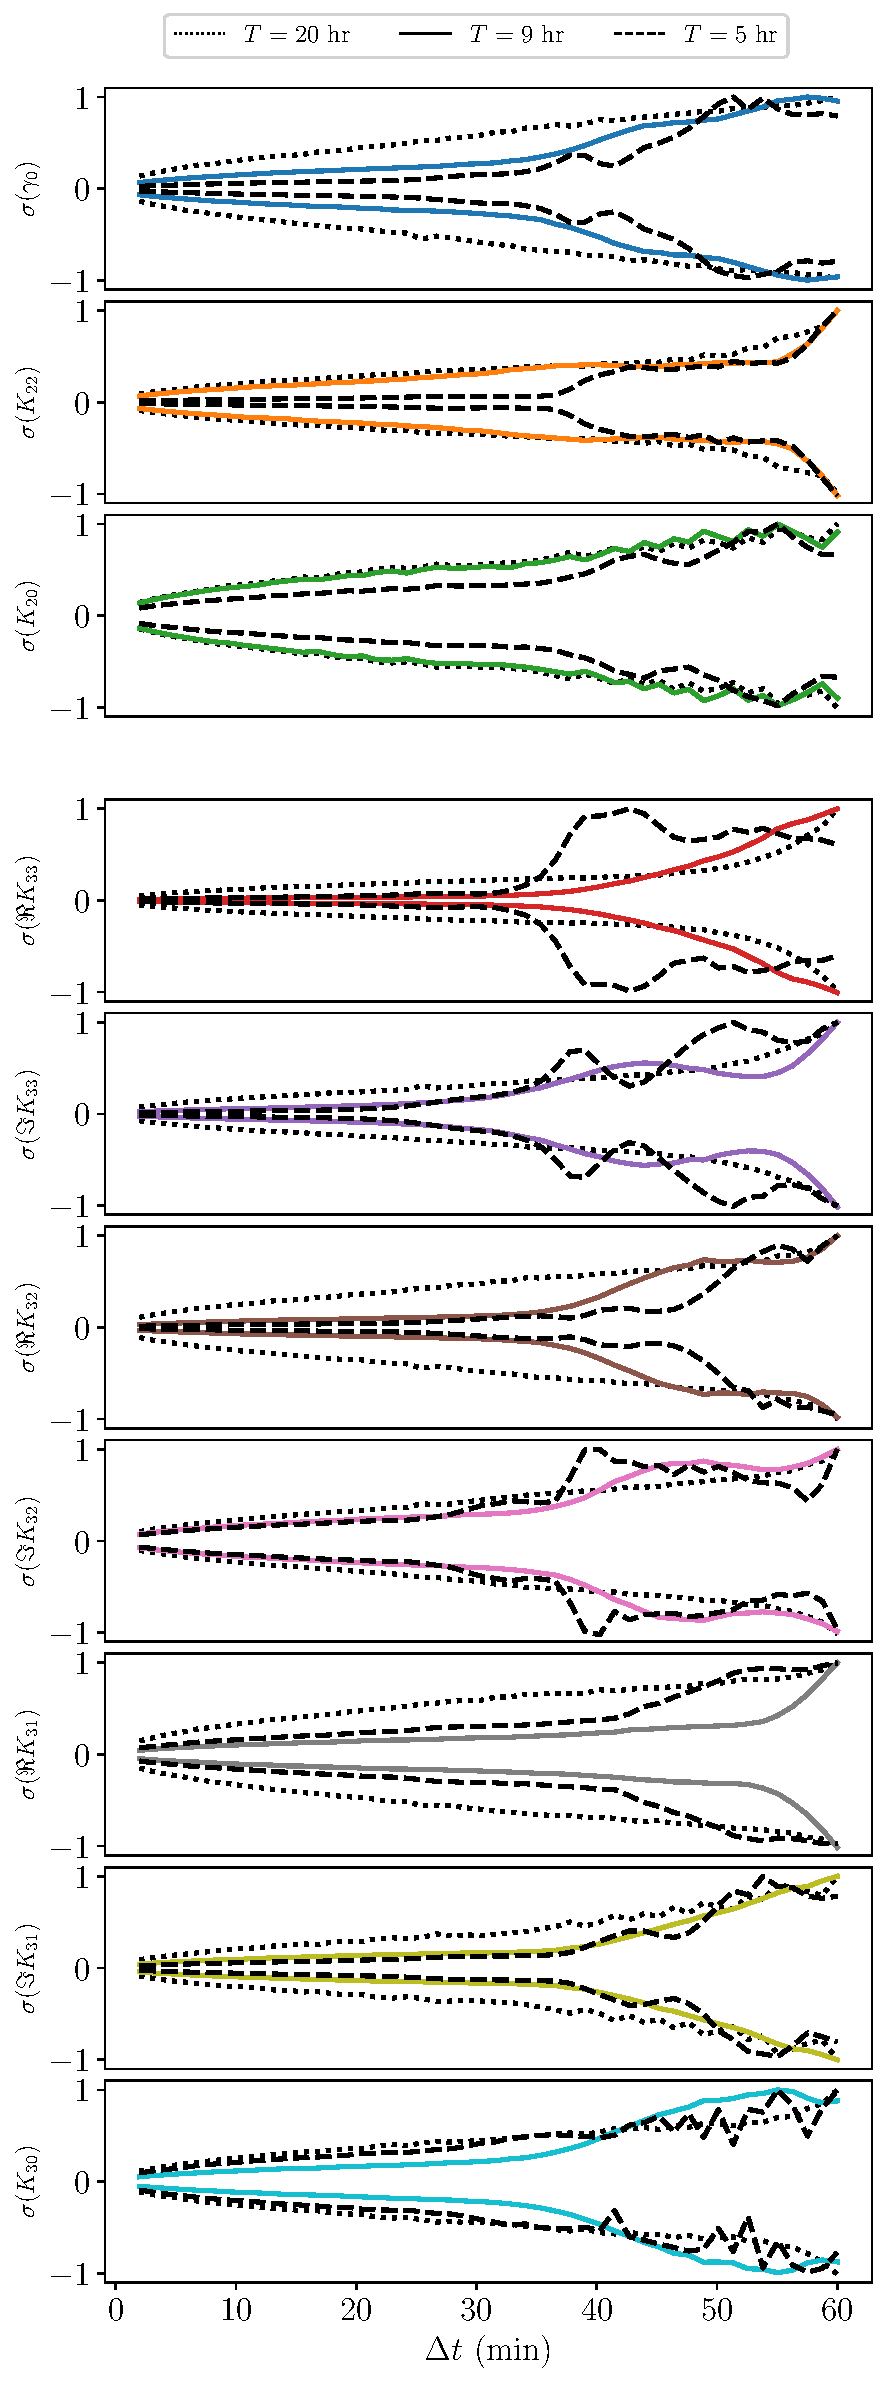
\includegraphics[width=0.48\textwidth]{figs/cad-period.pdf}\hfill
  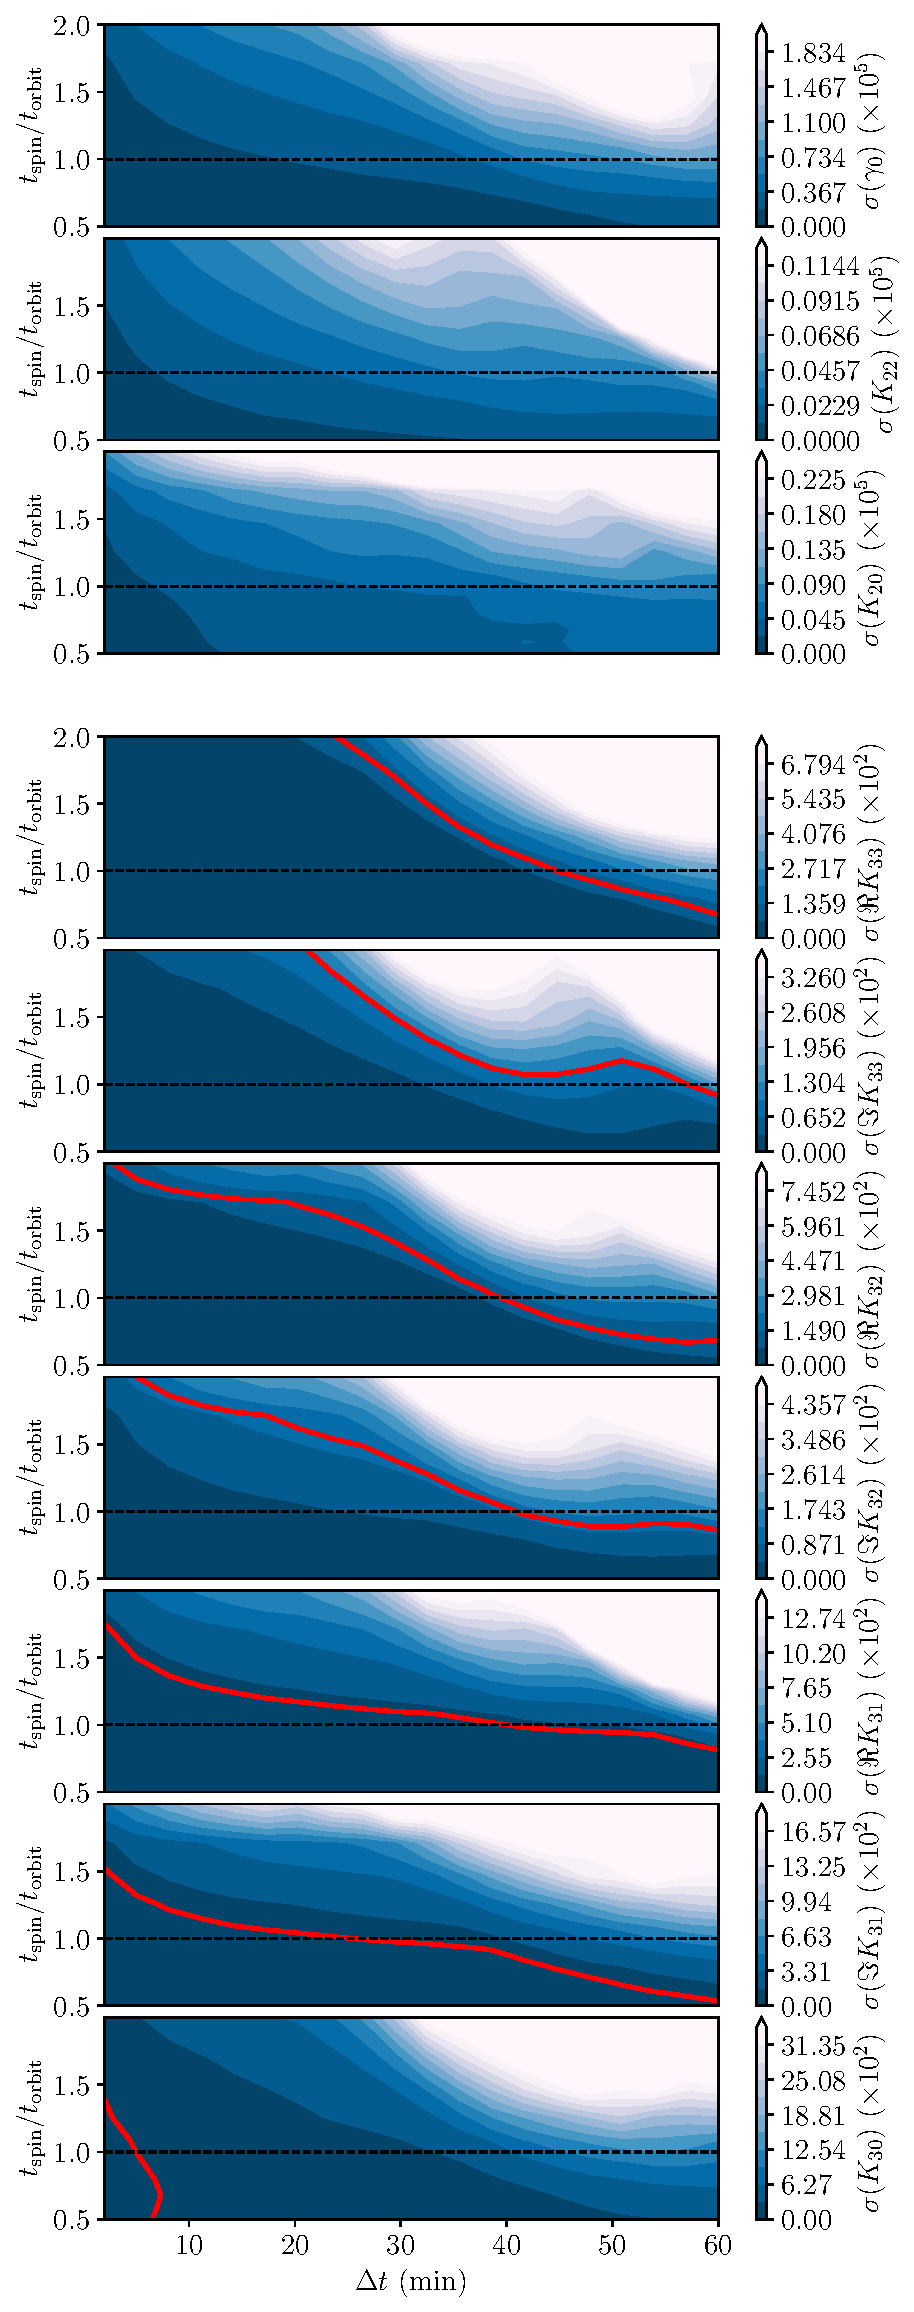
\includegraphics[width=0.48\textwidth]{figs/cad-speed.pdf}
  \caption{Contour plots showing posterior uncertainties as a function of cadence $\Delta t$ and dynamical time scales for the encounter: rotational period $P_\omega$ (\textit{left}) and the relative speed of the orbit (\textit{right}; see text for a definition). The reference values of $P_\omega=9$ hr and $t_\text{spin}/t_\text{orbit}=1$ are shown as dotted lines. The solid (dotted) red line represents the $\sigma_\rho / \rho = 100\%$ (20\%) threshold. Cadence cut-off depends strongly on both $P_\text{omega}$ and $t_\text{spin}/t_\text{orbit}=1$.}
  \label{fig:cad-contour}
\end{figure*}

Figure \ref{fig:cad-contour} demonstrates that large rotational period produces high $T_\text{cad}$. The dependence on $P_\omega$ agrees with the fact that large rotational periods for fixed cadence lead to better posterior uncertainty, discussed in section \ref{sec:scan-period}. The figure also demonstrates that for large $P_\omega$, $T_\text{cad}$ depends less strongly on $P_\text{omega}$ and may even reverse its dependence such that increasing $P_\text{omega}$ decreases $T_\text{omega}$. In all cases except $\Re K_{33}$, at least constant-$\sigma(K_{\ell m})$ contour is seen to curve back such that $\Delta t$ decreases as a function of $P_\text{omega}$ for large $P_\text{omega}$. In these regions the cadence cut-off also dulls, as shown by the spreading of the constant-$\sigma(K_{\ell m})$ contours in this region.

 The relative orbit speed $t_\text{spin} / t_\text{orbit}$ was defined by un-physically increasing or decreasing the time at which the asteroid moved through the orbit determined by the equations of motion (but leaving the orbit shape unchanged). The equations of motion affecting the orientation and spin of the asteroid however were unaffected. $t_\text{spin} / t_\text{orbit} > 1$ corresponds to a faster orbit, and $t_\text{spin} / t_\text{orbit} < 1$ corresponds to a slower orbit. With this unphysical process, we isolate the effect of the amount of time spent near perigee on posterior uncertainty, without inheriting additional affects that would have been caused by the orbit changing shape.

The right panel of figure \ref{fig:cad-contour} shows a stronger and more monotonic dependence of $T_\text{cad}$ on $t_\text{spin} / t_\text{orbit}$. It appears that even slightly slower orbits sharply increases $T_\text{cad}$. This effect is both due to the asteroid spending greater time in the high-torque, near-perigee region, and the larger data set that can be collected for slow orbits. However, if the orbit speed is changed by adjusting its parameters ($v_\infty$, $r_p$) or the central body mass $\mu_\mathcal{B}$, then the orbit shape will also change. This induces other effects studied in the main text and will complicate the trend observed here. Unlike the $P_\omega$ case, the cadence cut-off does not visibly broaden as a function of $t_\text{spin} / t_\text{orbit}$. It appears that the increased orbit speed merely shifts $T_\text{cad}$ rather than changing its sharpness.



\section{Uncertainty dependence on encounter properties}
\label{app:uncertainty-dependence}

\jtd{Review after thresholds.}

\begin{figure*}
  \centering
  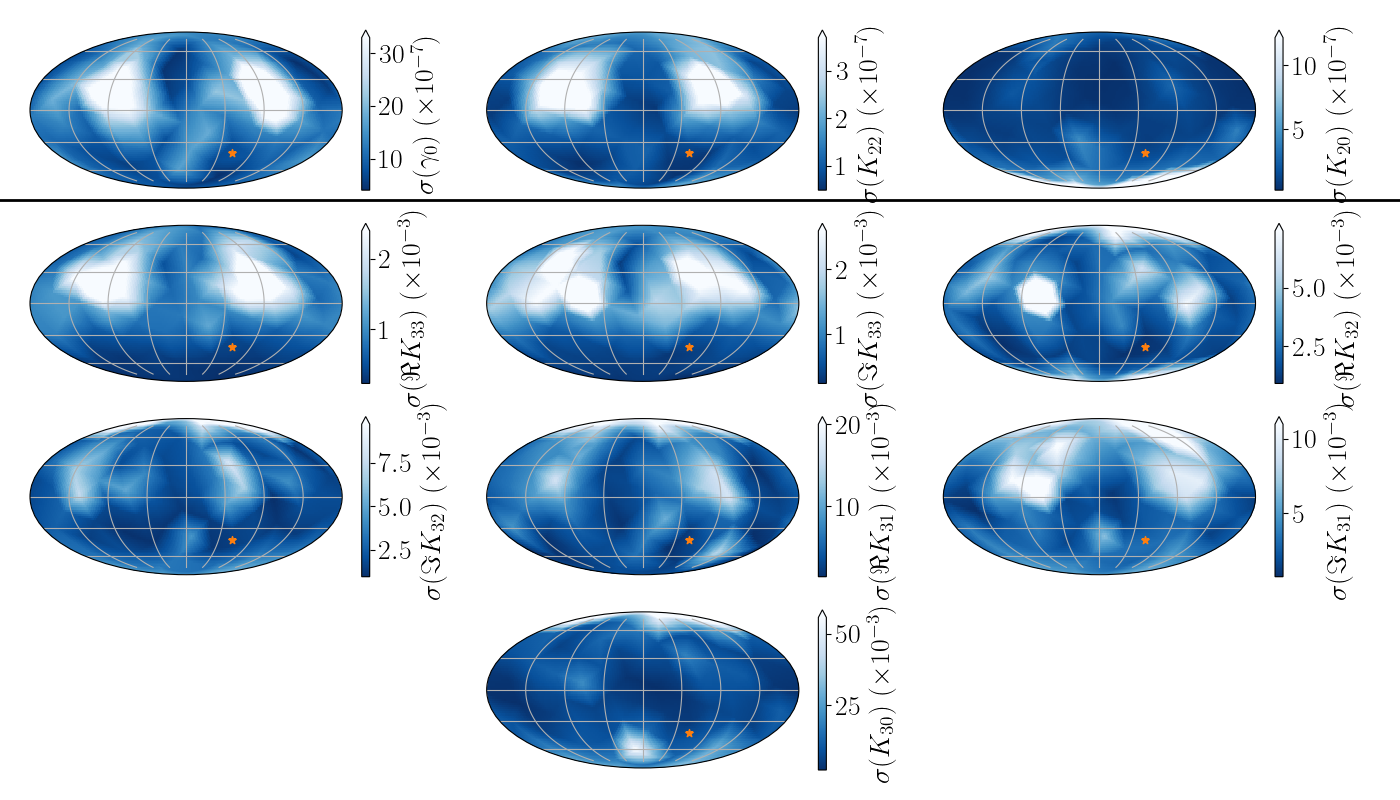
\includegraphics[width=0.8\textwidth]{figs/spin-pole.png}
  \caption{$1\sigma$ uncertainties for the first-order parameters (\textit{top}) and second-order (\textit{bottom}) as a function of the initial direction of spin in the inertial frame. All maps are made in the Mollweide projection. The orange star indicates the reference spin pole. The red contours enclose regions the 20\% (dotted) and 100\% (solid) $\sigma_\rho / \rho$ cut-off. Posterior uncertainty depends similarly on initial spin pole direction for all parameters}
  \label{fig:scan-spin}
\end{figure*}

In this section, we investigate in greater detail the data presented in section \ref{sec:fit-uncertainty} of the main text.

\subsection{Orbital elements}
\label{sec:scan-orbit}
A Keplerian orbit is completely described by five parameters, but three describe the orbit's orientation with respect to the central body. They are therefore redundant with the orientation of the inertial frame and we do not investigate them here. We parametrize the remaining two parameters by the perigee distance $r_p$ and excess velocity $v_\infty$. Fits of the type described in section \ref{sec:fit} were run for many values of $r_p$ and $v_\infty$ and the 1 and 2$\sigma$ posterior uncertainties are displayed in figure \ref{fig:scan-vex}.

Figure \ref{fig:scan-vex} demonstrates that posterior uncertainty follows a slight trend for uncertainty to increase with $v_\infty$. This is likely due to the fact that larger $v_\infty$ leads to a faster and flatter orbit with less time spent close to the planet, where tidal torque is strongest. There are also comparatively large oscillations in the uncertainty, due to the orientation of the asteroid at perigee varying. (The asteroid is always simulated to start at the same orientation, but increasing $v_\infty$ decreases the time to perigee so that the asteroid enters this region of high torque at different orientations depending on $v_\infty$.) Hence, the oscillations have the same period for all parameters.


The figure shows much stronger dependence of parameter uncertainty on perigee distance, as expected by the factor of $(a_\mathcal{A}/D)^{\ell'}$ present in equation \ref{eqn:tidal-torque} and mentioned in section \ref{sec:tidal-torque}. For $r_p =7.9$ Earth radii, $\sigma_\rho/\rho$ reaches the 100\% threshold. The 20\% threshold is reached at lower 4.7 Earth radii. Much of this uncertainty is dominated by uncertainty in $K_{30}$, which is the parameter least constrained by tidal torque analysis. At $r_p \approx 10$ Earth radii, $K_{30}$ fills the prior distribution with uncertainty ranging from -1 to 1, visible by the sudden cut-off in uncertainty increase and the discontinuity of the $\sigma(K_{\ell m})$ curve there.

The axes of figure \ref{fig:scan-perigee} show that parameters with large $m$ are more precisely determined than parameters with small $m$, as can be seen by comparing $K_{22}$ to $K_{20}$ and comparing $K_{33}$ to other $K_{3m}$ values. Large $m$ moments correspond to moments that control higher frequency fluctuations in density at the asteroid equator. This pattern of $\sigma(K_{\ell m})$ smaller for large $m$ is a general trend and will be seen in the following sections as well.

The very strong dependence of $\sigma(K_{\ell m})$ on $r_p$ makes this analysis most useful to extract second-order moments on close encounters. Fortunately, in the case of Earth, these encounters are also likely to have the best associated observational uncertainty when above the horizon due to their proximity. The first-order moments can still be extracted at much larger perigee distances in our model.


\subsection{Observational uncertainty}
\label{sec:scan-uncertainty}
Two parameters, $\sigma_\theta$ and $\sigma_\rho$, govern the observational uncertainty of the data set. These parameters are defined in section \ref{sec:uncertainty}; $\sigma_\theta$ represents the standard deviation of the angle between the true spin pole and the observed spin pole, while $\sigma_\rho$ represents the standard deviation of the ratio between the observed and true rotational velocities. Rather than explore the full space spanned by these two values, we fix one and allow the other to vary to better assess whether uncertainty in spin pole or uncertainty in period more strongly affects posterior uncertainty $\sigma(K_{\ell m})$. This dependence is displayed in figure \ref{fig:scan-theta}.

For the case in which $\sigma_\rho$ is held fixed and $\sigma_\theta$ is varied, the figure shows that the dependence of $\sigma(K_{\ell m})$ on $\sigma_\theta$ is linear. The uncertainty threshold is reached at $\sigma_\theta = 2.8^\circ$ (0.5$^\circ$) for $\sigma_\rho / \rho=$100\% (20\%). The $K_{2m}$ uncertainties remain low, even for $\sigma_\theta \approx 1$, which is large enough that the spin pole has non-negligible probability to be observed in any direction.

If $\sigma_\rho$ is allowed to vary instead, then $K_{30}$ reaches the 100\% and 20\% thresholds at $\sigma_\rho$ which correspond to period uncertainty of several milliseconds. At large period uncertainty, the PPDs begin to fill the prior and the posterior uncertainty $\sigma(K_{\ell m}$) is no longer linear with $\sigma_\rho$ (this is especially visible in the $K_{30}$) case. Otherwise, posterior uncertainty is proportional to $\sigma_\rho$.

These data show that posterior uncertainty is extremely sensitive to observational uncertainty in period in our analysis. To precisely measure density moments, very accurate rotational period estimates would have to be made for every angular velocity data point. However this analysis does not study the effect of collecting more data after the encounter, or the correlations between different angular velocity measurements. If these correlations were taken into account, or a more accurate uncertainty model used which took into account the asteroid's location in the sky or its distance to Earth, then the precision limit we find here will be affected.


\subsection{Asteroid shape}
\label{sec:scan-shape}

The true values of $K_{\ell m}$ and $a_\mathcal{A}$, which quantify the asteroid's physical properties, affect the posterior uncertainties. Here, we only investigate the sensitivity of $\sigma(K_{\ell m})$ to the first-order parameters and $a_\mathcal{A}$. These $K_{2m}$ moments can also be viewed as the axes of a uniform density triaxial ellipsoid (equation \ref{eqn:ellipsoid-axes}).

In figure \ref{fig:scan-space-sigma}, we show the 1$\sigma$ posterior uncertainties as a function of $K_{20}$ and $K_{22}$, or alternatively $a/c$ and $b/c$. We use axis ratios rather than the values of $a$, $b$, and $c$ because axis ratios are independent of $a_\mathcal{A}$. The large $|K_{22}|$ sides of the $K_{2m}$-space plots correspond to asymmetric ellipsoids, as do the points far from the $a/c=b/c$ diagonal of the axis-ratio-space plots. The point corresponding to a sphere, which experiences no tidal torque and no tumbling, is at $K_{2m}=0$ and $a/c=b/c=1$.

The figure shows large uncertainty in $\gamma_0$ for $K_{22}=0$, or $a/c=b/c$, because $K_{20}$ is rotationally symmetric around $\unit z$, and $\gamma_0$ is the initial orientation with respect to the $\unit z$ axis. The system then has no dependence on $\gamma_0$ when $K_{22}=0$. This induces degeneracy in the model which inflates uncertainties, not only in $\gamma_0$ but also the other components.

To remove the inflated uncertainty, one could assume a rotationally symmetric asteroid, remove $\gamma_0$ as a parameter, and run a fit. For a nearly rotationally symmetric asteroid however, a new parametrization is necessary which does not contain the ill-constrained $\gamma_0$ parameter. This task is beyond the scope of this paper, so we mostly consider asymmetric asteroids throughout.

Figure \ref{fig:scan-space-sigma} also shows low uncertainty for highly asymmetric asteroids, where $b/c$ and $a/c$ are very different (i.e., when $|K_{22}|$ is large). Additionally, $\sigma(K_{20})$ and $\sigma(K_{22})$ decrease for large $|K_{20}|$, which corresponds to large axis ratios in the ellipsoid case.

Figure \ref{fig:scan-space-corr} displays the correlation between the first-order parameters. They show that $\gamma_0$ and $K_{22}$ are often correlated for asymmetric asteroids, while $\gamma_0$ and $K_{20}$ are usually not. This is expected as $K_{22}$ is dependent on the orientation of the asteroid and $K_{20}$ is not. They also show that $K_{22}$ and $K_{20}$ are usually correlated, and that $a/c$ and $b/c$ are highly correlated. The latter is expected due to the $1/c$ dependence.

\begin{figure*}
  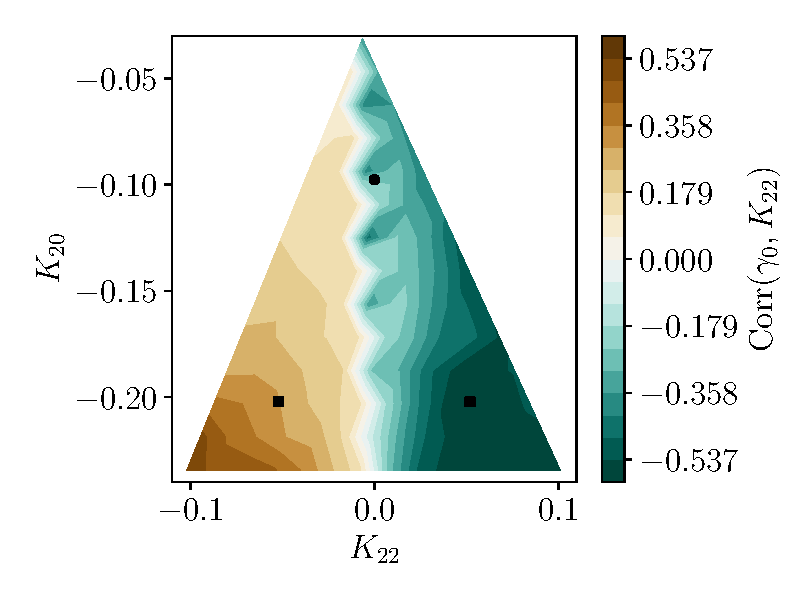
\includegraphics[width=0.3\textwidth]{figs/probe-space-corr12.pdf}\hfill
  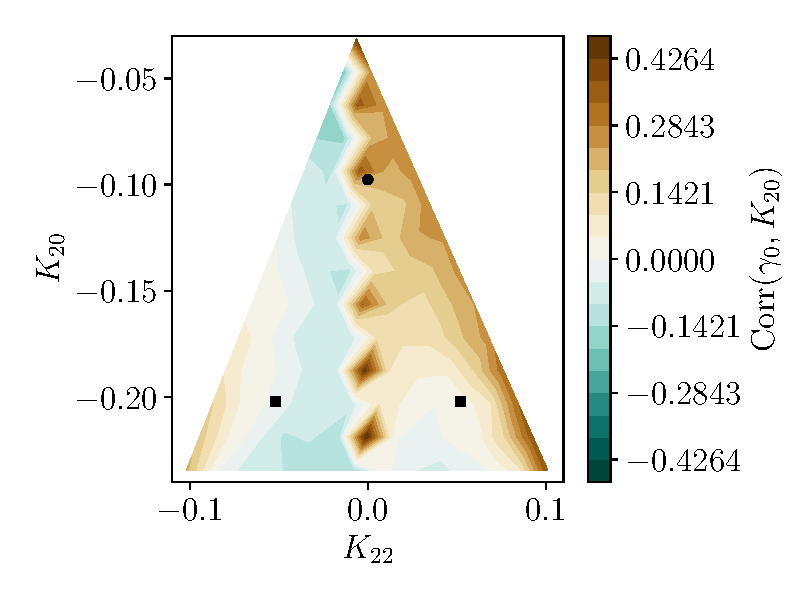
\includegraphics[width=0.3\textwidth]{figs/probe-space-corr13.pdf}\hfill
  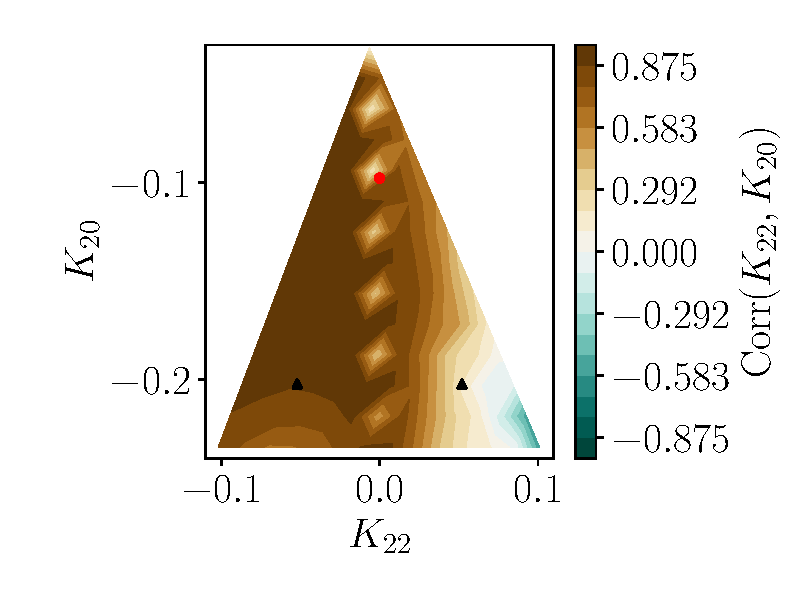
\includegraphics[width=0.3\textwidth]{figs/probe-space-corr23.pdf}

  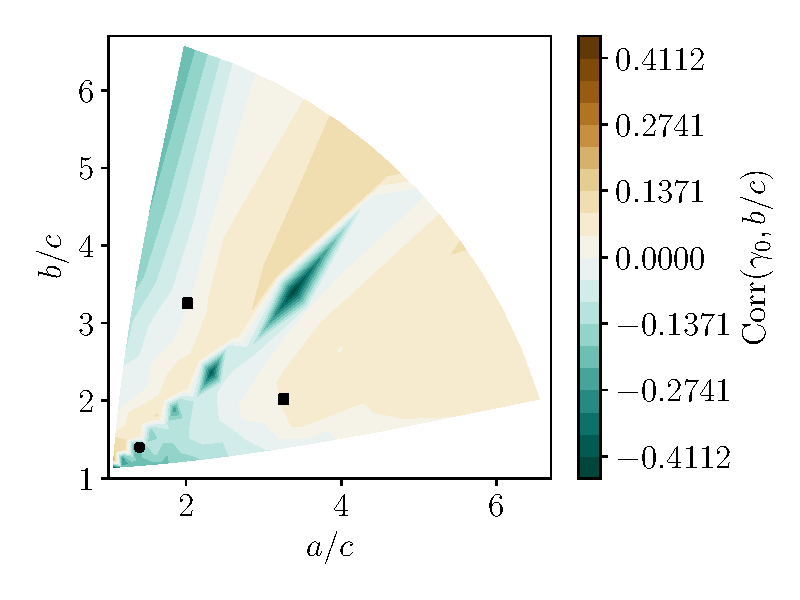
\includegraphics[width=0.3\textwidth]{figs/probe-space-ab-1b.pdf}\hfill
  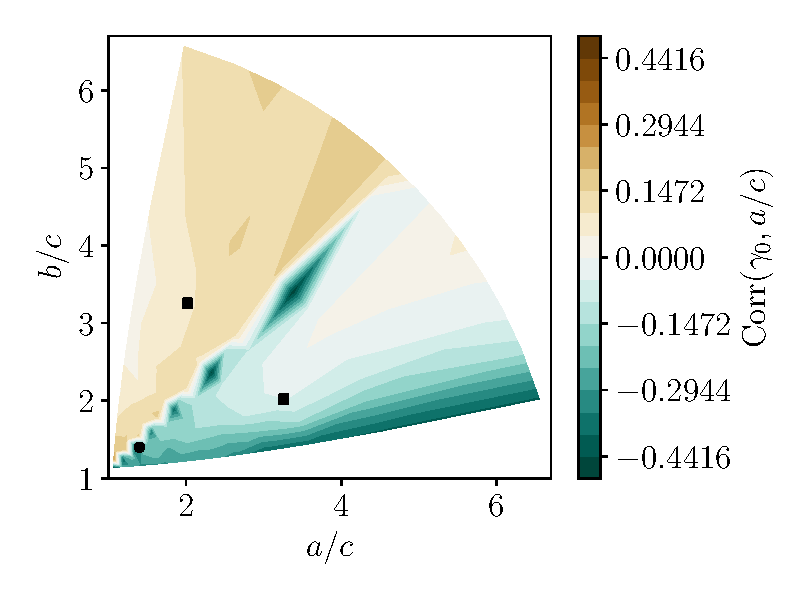
\includegraphics[width=0.3\textwidth]{figs/probe-space-ab-1a.pdf}\hfill
  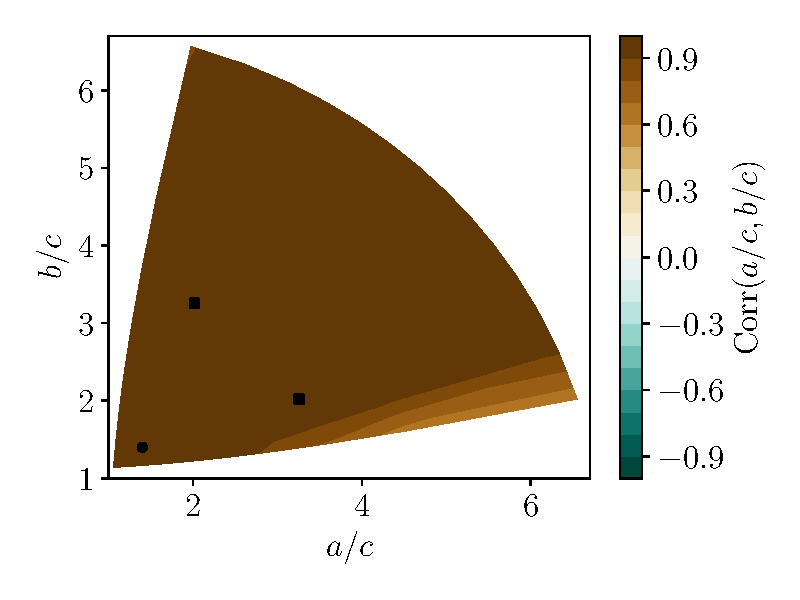
\includegraphics[width=0.3\textwidth]{figs/probe-space-ab-ab.pdf}
  
  \caption{Correlations between PPDs for first-order parameters $\gamma_0$, $K_{22}$, and $K_{20}$ (\textit{top row}) and $\gamma_0$, $a/c$, and $b/c$ (\textit{bottom row}).  Also shown as black points are the reference asteroid shapes: symmetric (red circle) and asymmetric (black triangle). The first order parameters $K_{22}$ and $K_{20}$ are correlated, as are initial orientation $\gamma_0$ and $K_{22}$.}
  \label{fig:scan-space-corr}
\end{figure*}

The fact that $K_{\ell m}$ are correlated indicates that, in order to correctly propagate density moment uncertainties to a density distribution, a full PPD is necessary. If only 1$\sigma$ uncertainty intervals for each parameter were used, density distribution uncertainty would be overestimated. This full PPD is produced by our fit process, but only the 1$\sigma$ uncertainties are displayed in this paper in most cases.

Overall, the variation in the uncertainties on $K_{20}$ and $K_{22}$ (the first-order density moments) is present but largely smooth across their allowed parameter space, as is their correlation. It therefore seems reasonable to use the asymmetric asteroid shape as a stand-in for an unknown's asteroid shape when simulating an encounter, as we do in this paper. The uncertainty then can be expected to differ across other shapes by a factor of about two or less, as long as the degenerate, symmetric asteroid regime is avoided.

On the other hand, the posterior uncertainty of $K_{3m}$ is much more strongly dependent on asteroid length $a_\mathcal{A}$. Figure \ref{fig:scan-am} displays posterior uncertainty $\sigma(K_{\ell m})$ as a function of $a_\mathcal{A}$. As was mention in section \ref{sec:tidal-torque}, the $K_{2m}$ parameters are insensitive to $a_\mathcal{A}$ since the $a_\mathcal{A}^2$ term in $\bm \tau$ (equation \ref{eqn:tidal-torque}) cancels the $a_\mathcal{A}^2$ in the MOI (equation \ref{eqn:moi}). The $K_{3m}$ uncertainty is strongly dependent on $a_\mathcal{A}$ for the same reason that it is dependent on $r_p$: the $(a_\mathcal{A}/D)^{\ell'}$ dependence of equation \ref{eqn:tidal-torque}. At $a_\mathcal{A} \leq 1100$ m, $\sigma_\rho/\rho \approx 100\%$. However, the 20\% cut-off is much lower, at $a_\mathcal{A} \leq 180$. Figure \ref{fig:scan-am} demonstrates why these cut-offs are so distant; for large $a_\mathcal{A}$, uncertainty decreases slowly with length. Only for small lengths is the uncertainty very large. This behaviour indicates that the uncertainty threshold is unlikely to fall much below 180 m even if other properties of the encounter are adjusted.

For uniform density asteroids, large $a_\mathcal{A}$ is equivalent to large asteroid radius. In non-uniform density asteroids, large $a_\mathcal{A}$ can also be achieved by distributing the mass of the asteroid near the surface, because the $r^2$ term in the integrand of the definition of $a_\mathcal{A}$ causes the density of regions distant from the asteroid centre of mass to dominate $a_\mathcal{A}$.




\subsection{Cadence}
\label{sec:scan-cadence}

The time between observations of asteroid angular velocity, or cadence, may vary depending on the observational schedule of the observing telescopes and the path of the asteroid through the sky.  We measure how the posterior uncertainty $\sigma(K_{\ell m})$ varies with cadence ranging from two minutes to one hour in figure \ref{fig:scan-cadence}.

Figure \ref{fig:scan-cadence} displays little dependence of uncertainty on cadence $\Delta t$ for $\Delta t \lesssim 40$ min. We also see flaring of uncertainty for very large cadence, largely driven by the paucity of data points. However, uncertainty dramatically increases for many parameters at about $\Delta t = 30-40$ min, a time scale which is likely characteristic of the asteroid system.  We name this rough cadence limit $T_\text{cad}$. $T_\text{cad}$ is also the location at which the $\sigma(K_{3m}$ threshold is crossed for all second-order moments except $K_{30}$, which exceeds the uncertainty threshold at $\Delta t \approx 5$ min.

We expect this $T_\text{cad}$ to be a function of two dynamical time scales of the system: the rotational period of the asteroid $P_\omega$ and the dynamical time scale of the orbit (the latter can be estimated in multiple ways, since both $r_p / v_\infty$ and $v_\infty r_p^2 / \mu_\mathcal{B}$ have units of time and may be relevant). How these time scales affect $T_\text{cad}$ is discussed in appendix \ref{app:cadence-tests}.

Figure \ref{fig:scan-cadence} shows that as long as $\Delta t < T_\text{cad}$ is achieved, the influence of cadence on $\sigma$ is minimal, but shorter cadence leads to lower uncertainties.



\subsection{Perigee gap}
\label{sec:scan-gap}
In certain circumstances, spin data might not be able to be captured for a close encounter at perigee. The asteroid might dip below the horizon, or it might pass too close to the sun to be observed. Generally, angular velocity data can be collected when the asteroid is distant from the central body, where torque is low. There, the angular velocity evolution is dominated by torque-free precession dictated by the MOI components. That zero-torque data can still be used to fix $K_{20}$ and $K_{22}$ as in \cite{MOSKOVITZ2020113519}. However, $K_{3m}$ does not affect the precession periods (though they do affect the phase). We are therefore curious as to how our posterior uncertainties change due to lack of perigee data.

To test this, we mask the perigee of the counter by removing a duration $T_\text{gap}$ of data centred on the perigee, where $T_\text{gap}$ ranges from 0 to 3 hours. To prevent lack of precision on $K_{\ell m}$ induced by lower amounts of data for high $T_\text{gap}$, we always cut 3 hr$-T_\text{gap}$ from the data set, half from the beginning and half from the end, so that each data set produced for all $T_\text{gap}$ has the same size. We then fit the same asteroid model to the cut data for all $T_\text{gap}$ and plot posterior uncertainties $\sigma(K_{\ell m})$ in figure \ref{fig:observation-gap}.

Since torque is greatest at perigee, we expect that region of the data to contain the most information about $K_{\ell m}$, and therefore uncertainty should increase monotonically with $T_\text{gap}$, which is seen in figure \ref{fig:observation-gap}. We also see that the first-order parameters are not as sensitive to $T_\text{gap}$ as the second-order parameters, because $K_{2m}$ are additionally constrained by torque-free precession after perigee.

Most parameters show dramatically increased uncertainty in the $T \sim 1-2$ hr range. On the other hand, none of the uncertainties increase noticeably for $T \lesssim 1$ hr. Thirty minutes of dropped data is equivalent to fifteen dropped points for the simulated cadence of $\Delta t = 2$ minutes, showing that many data points can dropped from the data set at perigee before the uncertainty starts to increase.

Qualitatively, \ref{fig:observation-gap} shows similar dependence of $\sigma(K_{\ell m})$ on $T_\text{gap}$ as on cadence $\Delta t$; they also both have cut-offs where uncertainty markedly increases, and both the $T_\text{gap}$ and $\Delta t$ cut-offs have qualitatively similar shapes although they occur at different values of $\Delta t$ and $T_\text{gap}$. This suggests that the factors that govern uncertainty due to cadence also may govern sensitivity to lack of data at perigee in a similar way.


\subsection{Initial spin pole}
\label{sec:scan-spin}

The tidal torque experienced by the asteroid is affected by the initial direction of asteroid spin $\bm \Omega_0$ both because spin sets the initial asteroid orientation up to $\gamma_0$ and because of the spin-dependence of the rotational equations of motion (equation \ref{eqn:omega-eom}).

In figure \ref{fig:scan-spin}, we display 1$\sigma$ posterior uncertainties as a function of the direction of $\bm \Omega_0$ mapped onto the unit sphere in the inertial frame. Our samples for $\bm \Omega_0$ were laid out on a Fibonacci sphere to ensure they were roughly evenly spaced (marked in figure \ref{fig:scan-spin-avg}). To highlight common features across the parameters, we also display the average 1$\sigma$ sensitivity in figure \ref{fig:scan-spin-avg}. The average is weighted such that the uncertainty map for each parameter contributes an equal amount (the weight of each map is set to one-tenth of the map's mean). This average map is presented in two different projections to allow data at $\unit Z$ to be read.

\begin{figure*}
  \centering
  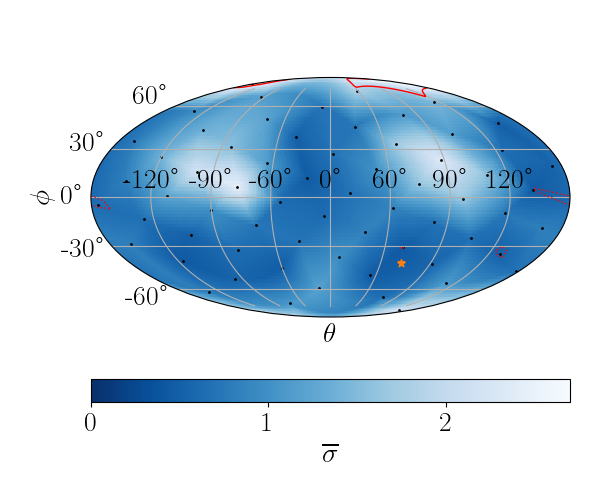
\includegraphics[width=0.3\textwidth]{figs/spin-pole-avg-mollweide.png}
  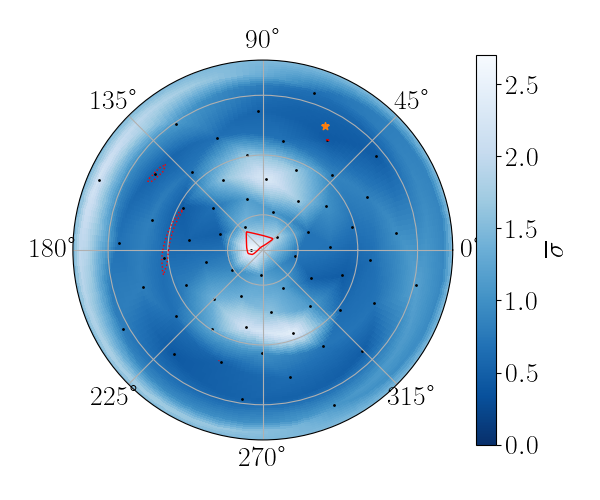
\includegraphics[width=0.3\textwidth]{figs/spin-pole-avg-polar.png}
  \caption{The weighted average of the uncertainties shown in figure \ref{fig:scan-spin}, in Mollweide (\textit{left}) and polar (\textit{right}) projections in the inertial frame. See text for a description of how the average was computed. Black dots indicate the Fibonacci-sphere-distributed locations of sample spin poles, and the orange star indicates the reference spin pole. The polar projection is centred at the north pole, or $\unit Z$. Posterior uncertainty is large near $\pm \unit Z$ and $\pm \unit Y$, but roughly constant elsewhere.}
  \label{fig:scan-spin-avg}
\end{figure*}

Certain alignments of the body-fixed frame to the inertial frame lead to special conditions on torque, as discussed in section \ref{sec:tidal-torque}. For example, $\bm z \parallel \unit Z$ and $\bm z \parallel \unit Y$ at perigee lead to $\bm \tau \parallel \unit z$ to first-order, and $\bm \tau \parallel \unit X$ at perigee leads to $\bm \tau = 0$ to first-order. We relate this to the initial direction of $\bm \Omega_0$, via the approximation that $\bm \tau$ is small until perigee. Then $\bm \Omega_0 \parallel \unit Y$ and $\bm \Omega_0 \parallel \unit Z$ both lead to $\bm \tau \parallel \unit z$, and $\bm \Omega_0 \parallel \unit X$ leads to $\bm \tau = 0$.

Figure \ref{fig:scan-spin-avg} shows area of increased uncertainty for $\bm \Omega_0 \parallel \unit Z$ and $\bm \Omega_0 \parallel \unit Y$, but not the $\unit X$ case. This indicates that $\bm \tau \parallel \unit z$ causes increased uncertainty. Physically, $\bm \tau \parallel \unit z$ only changes an asteroid's rotational period and does not cause it to tumble, eliminating the ability to discern MOI ratios from zero-torque precession after the encounter. If $\bm \tau = 0$ to first-order, then second-order $\bm \tau$ and non-perigee $\bm \tau$ will dominate, which may increase precision to these usually non-dominant parameters and therefore not have the same increasing effect on $\sigma(K_{\ell m})$.

However, uncertainty does not vary by much more than a factor of two outside the imprecise regions of $\bm \Omega_0 \parallel \unit Z$ and $\bm \Omega_0 \parallel \unit Y$, though these regions are wide for some parameters. Within the imprecise regions, uncertainty can grow up to four times or more the uncertainty at other $\bm \Omega_0$ values, and can exceed the $\sigma(K_{3 m}) \approx 0.01$ threshold. The trends for are roughly consistent across parameters (figure \ref{fig:scan-spin}), leading to clearly visible imprecise regions in the average $\sigma(K_{\ell m})$ (figure \ref{fig:scan-spin-avg}).



\subsection{Rotational period}
\label{sec:scan-period}

We also study the effect of the initial rotational period of the asteroid $P_\omega$ on posterior uncertainty $\sigma(K_{\ell m})$. In figure \ref{fig:scan-period}, we show $\sigma(K_{\ell m})$ as a function of $P_\omega$ for a range of periods typical of NEOs. Like figure \ref{fig:scan-vex}, depicting the dependence of $\sigma(K_{\ell m})$ on $v_\infty$, figure \ref{fig:scan-period} shows small-scale variation in uncertainty due to the fact that varying the initial period changes the value of $\gamma$ at perigee, which affects uncertainty to a factor of about two. But a large-scale trend is also visible in many parameters. $K_{20}$ and $K_{22}$ show very large uncertainty for $P_\omega \lesssim 4$ hr because these fast-rotators tumble very little after perigee. This increases uncertainty on the $K_{2m}$ parameters, which are constrained by tumbling.

We expect that quickly rotating asteroids would not tumble because, for small $P_\omega$, the dynamical variables $\bm D$, $\bm \omega$, $\alpha$, and $\beta$ vary much smaller than $\gamma$. Approximating each variable as constant over one full rotation of $\gamma$, we can integrate the first-order contribution of $\bm \tau$ over $\gamma \in (0, 2\pi)$, which gives no secular, first-order torque to force the asteroid to tumble. However, this effect does not apply to the second-order parameters, since the integral over the second-order term of $\bm \tau$ does not vanish, as seen in the figure.

Another feature of figure \ref{fig:scan-period} is that $K_{\ell 0}$ is more uncertain at low $P_\omega$ than the other parameters. This is most visible in the figure for $K_{30}$. The cause is likely that $K_{\ell 0}$ cannot contribute to $\tau_z$ as shown in equation \ref{eqn:tidal-torque}. We already discussed that asteroids with small $P_\omega$ do not tumble, and since $\tau_x$ and $\tau_y$ are what induces tumbling, the most observable component of torque is therefore $\tau_z$, which $K_{\ell 0}$ do not affect.

The most severe effect of period on $\sigma(K_{\ell m})$ is in the low-period regime ($P_\omega < 4.3$ hr), but in this case, the most strongly affected parameters are $K_{2m}$, which are generally known better than $K_{3m}$. The effect on the imprecise parameters $K_{3m}$ is small, except for $K_{30}$. It therefore seems as though small-period asteroids are still candidates for observation, although high-period asteroids yield smaller uncertainty.


\subsection{Central body oblateness}
\label{sec:scan-oblateness}

In all the above studies, we assumed a spherical planet ($J_{\ell m} = 0$ for $\ell \geq 1$). By assumption that $\mu_\mathcal{B} \gg \mu_\mathcal{A}$ (so that the asteroid orbit's focus is the centre of mass of the central body), we have $J_{1m} = 0$. The effect of central body non-sphericity, then, is limited to the $J_{2m}$ terms and damped by a factor of $(a_\mathcal{B} / D)^2$. We expect these parameters to have small effect on the asteroid.

Here, we define oblateness as $\epsilon = (I_z - I_x)/(\mu_\mathcal{B} R_\mathcal{B}^2)$, where $I_{x,y,z}$ are the central body moments of inertia along the principal axes, and $I_x = I_y$. $R_\mathcal{B}$ is the true radius of the body (not $a_\mathcal{B}$ from equation \ref{eqn:jlm}). 

$J_{\ell m}$ is defined in equation \ref{eqn:jlm} with respect to the asteroid orbit, not the principal axes of the central body. However, for an equatorial orbit, the central body principal axes coincide with the asteroid orbit frame and we may express $\epsilon$ simply in terms of $J_{\ell m}$ as $\epsilon = -10J_{20}/3$ and $J_{22} = 0$. For simplicity, we use this equatorial orbit case. Since an oblate ellipsoid is mirror-symmetric around all three axes, table \ref{tab:klm-symmetries} indicates that $J_{3m}$ are all zero. The next order of tidal torque is therefore $J_{4m}$, damped by an additional $(a_\mathcal{B}/D)^2$ factor, and non-ellipsoid corrections to the central body shape. We do not consider these extra factors.

\begin{figure}
  \centering
  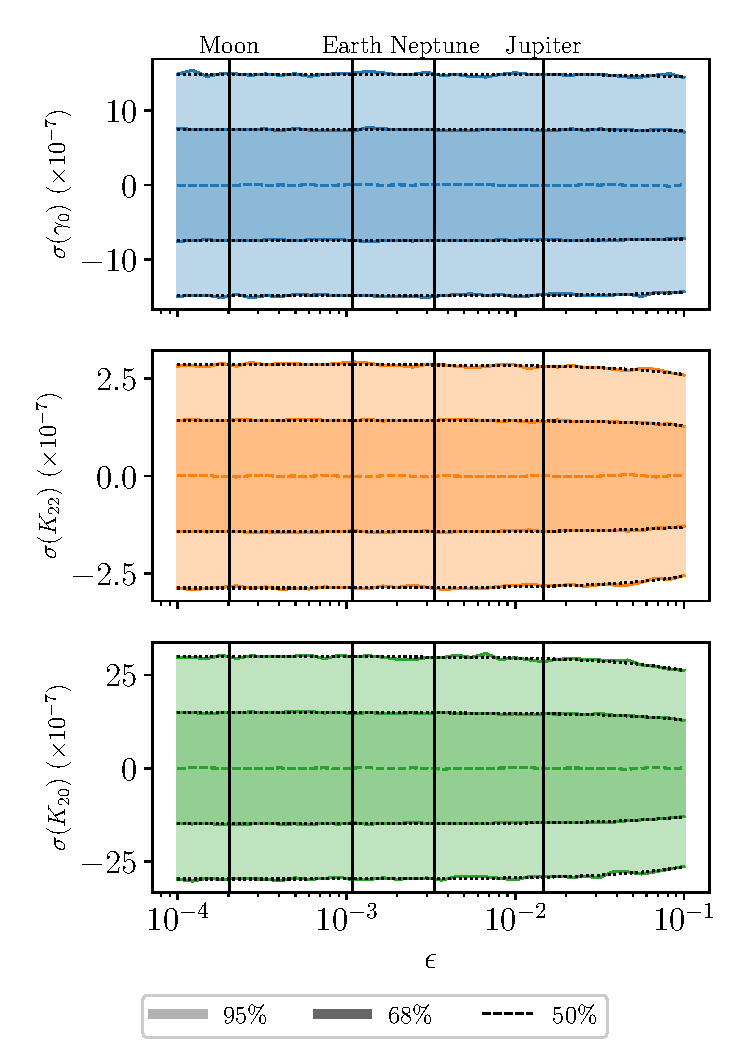
\includegraphics[width=0.88\columnwidth]{figs/oblateness.pdf}
  \vfill
  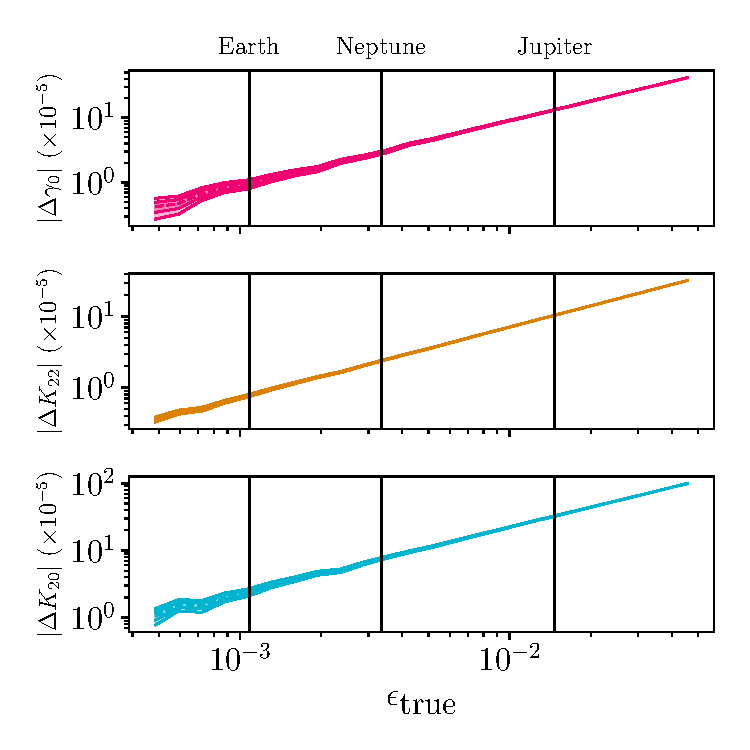
\includegraphics[width=0.88\columnwidth]{figs/oblateness-differ.pdf}
  \caption{\textit{Top}: 1 and 2$\sigma$ confidence intervals for the first-order parameter PPDs as a function of oblateness $\epsilon$ . Linear best-fitting lines to $\sigma(K_{2m})$ (black, dotted) are plotted. \textit{Bottom}: The difference between PPD means extracted from a zero-oblateness model and the true parameters given data with true oblateness $\epsilon_\text{true} \neq 0$. Also shown in both figures are the oblatenesses of reference Solar System bodies. Posterior uncertainty depends little on oblateness, but the best-fitting parameter estimates are affected enough by oblateness that oblateness must still be modelled.}
  \label{fig:scan-oblateness}
\end{figure}

Given this conversion between $\epsilon$ and $J_{20}$, we analyze posterior uncertainty $\sigma(K_{2 m})$ of the first-order parameters as a function of $\epsilon$ across a reasonable range of central body oblatenesses based on those of Solar System planets \cite{paterLissauer2015}. These uncertainties are shown in the top panel of figure \ref{fig:scan-oblateness}, together with linear best-fitting curves. The figure demonstrates almost no dependence of $\sigma(K_{\ell m})$ on oblateness $\epsilon$, although posterior uncertainty does measurably decrease for oblate central bodies. The best-fitting lines match the uncertainties well, and they have slope of $[\Delta \sigma(K_{\ell m}) / \sigma(K_{\ell m})_{\epsilon=0}] / \Delta \epsilon = -0.06$ for $\gamma_0$, $-0.2$ for $K_{22}$, and $-0.3$ for $K_{20}$. The second-order parameters $K_{3m}$ likely depend on oblateness similarly, but fitting these parameters is computationally more expensive and we do not study them.

Note that if an encounter is executed around one of the non-Earth objects noted in figure \ref{fig:scan-oblateness}, $a_\mathcal{B}$ and $\mu_\mathcal{B}$ will change in addition to $\epsilon$. These two parameters also affect the posterior uncertainty (section \ref{sec:jupiter-earth}), so the figure does not show that encounters with other bodies have the same precision as encounters with Earth; only that the difference in oblateness between the two bodies is of little concern.

Given the small effect of $\epsilon$ on $K_{\ell m}$, it might be tempting to neglect the planetary oblateness when fitting $K_{\ell m}$ to data. However, the bottom panel of figure \ref{fig:scan-oblateness} demonstrates that doing so is invalid. This figure displays $K_{\ell m}$ as extracted by a fit assuming $\epsilon = 0$, but run on data generated with non-zero $\epsilon$. The difference between the PPD means and true parameters are shown. Posterior uncertainties are also shown as bands. The figure shows that even for low (Earth-scale) oblateness, the fit results are inconsistent with the true $K_{\ell m}$ values, since $\Delta K_{\ell m} = 0$ is not contained in the 2$\sigma$ band. This effect is much worse for large oblateness, growing to a difference on the order of $\mathcal{O}(100)\sigma$ for Jupiter's oblateness. Therefore, accurately modelling central-body oblateness to high precision is essential for accurate estimation of fit parameters. For non-equatorial orbits, with $J_{22} \neq 0$, we also expect $J_{22}$ to affect the accuracy of the fit results to a similar degree, with the additional requirement of using the correct asteroid orbital plane.

$J_{20}$, the parameter studied in this section, has a slightly more general definition than oblateness. If the planet has a moon, the integral defining $J_{20}$ (equation \ref{eqn:jlm}) can be extended to include this extra mass, though this can only be done when the asteroid never passes inside the moon's orbit. As an order-of-magnitude estimate for this effect, two spherical objects with masses and radii of Earth and the Moon, separated by one Lunar distance, and both lying in the orbital plane has a combined oblateness of $\epsilon = 0.82$. Extrapolating posterior uncertainties via the slopes of the best fit lines given earlier yields a reduction in $\sigma(K_{2m})$ by about 25\%. Furthermore, $J_{22}$ is non-zero for this case, which likely decreases posterior uncertainty even more.

This analysis suggests that large moons such as ours can improve fit quality, but further study of this effect is beyond the scope of this paper. Without a moon to inflate the oblateness of the central body, planetary oblateness does not significantly improve posterior uncertainty. However, correct representation of oblateness is essential to accurately estimate $K_{\ell m}$.


\section{Animated density distributions}

This figure contains animations to better display the density distributions shown in the main text. Each frame represents a cross section perpendicular to the $\unit z$-axis, starting with negative $z$ and ending with positive $z$.

\begin{figure*}
  \textbf{Please see the published version of the paper for these animations, or find them online at the following links.}

  \href{}{}

  \caption{Density distributions extracted via the finite element model for the asymmetric (\textit{first and thrid row}) and symmetric (\textit{second and fourth rows}) reference asteroids. The finite element model (\textit{top two rows}) and the lumpy model (\textit{bottom two rows}) are employed. From left to right, the densities, deviations from the true density, uncertainties, and significance of the deviations are plotted. Animated form of figure \ref{fig:den-uniform}.}
  \label{fig:animated-uniform}
\end{figure*}

\begin{figure*}
  \textbf{Please see the published version of the paper for these animations}

  \caption{Density distributions extracted via the finite-element (\textit{top}) and lumpy (\textit{bottom}) models for an asteroid with a centred core. From left to right, the densities, deviations from the true density, uncertainties, and significance of the deviations are plotted. Animated form of figure \ref{fig:den-sph}.}
  \label{fig:animated-sph}
\end{figure*}

\begin{figure*}
  \textbf{Please see the published version of the paper for these animations}

  \caption{Density distributions extracted via the finite-element (\textit{top}) and lumpy (\textit{bottom}) models for an asteroid with an off-center core. From left to right, the densities, deviations from the true density, uncertainties, and significance of the deviations are plotted. Animated form of figure \ref{fig:den-move}.}
  \label{fig:animated-move}
\end{figure*}

\begin{figure*}
  \textbf{Please see the published version of the paper for these animations}

  \caption{Density distributions extracted via the finite-element (\textit{top}) and the two-lump lumpy (\textit{bottom}) models for an asteroid with two counterbalancing cores. From left to right, the densities, deviations from the true density, uncertainties, and significance of the deviations are plotted. Animated form of figure \ref{fig:den-double}.}
  \label{fig:animated-double}
\end{figure*}